\chapter{Superladungen, Abschluss und Superspace}

\lectureoverview{Supersymmetrie ist nicht deshalb schwierig, weil es viele Regeln gibt, sondern weil diese Regeln Ideen verbinden, die in der gewöhnlichen Physik getrennt bleiben. Wir beginnen mit Grassmann-Variablen, deren ungerade Elemente antikommutieren und deren Funktionen nach endlich vielen Termen abbrechen. Ihre Ableitungsalgebra liefert dann das Vorbild für ungerade Symmetrieerzeuger. Ein bosonischer und ein fermionischer Oszillator ergeben die einfachsten Superladungen: Ihr Antikommutator ist der Hamiltonoperator, sodass der Austausch von Bosonen und Fermionen untrennbar mit einer Zeittranslation verbunden ist. Dieselbe Algebra lässt sich geometrisch als Translationen in Grassmann-Richtungen einer erweiterten Raumzeit darstellen, die Superspace genannt wird.}

\section{Warum wir einen Schritt zurückgehen müssen, bevor wir vorankommen}

Die Supersymmetrie gehört zu den abstraktesten Konstruktionen der Physik. Als Symmetrie ähnelt sie Rotationen und Translationen, doch sie lässt sich nicht in die gewöhnliche Raumzeit einfügen, ohne unsere Vorstellung davon zu erweitern, was eine Koordinate ist. Ihre natürlichen Parameter sind Grassmann-Größen: Objekte, die sich addieren und multiplizieren lassen, aber antikommutieren statt zu kommutieren.

Deshalb wäre es wenig hilfreich, sich direkt mit der endgültigen Algebra auseinanderzusetzen. Zunächst machen wir die ungerade Arithmetik handhabbar, rufen uns dann in Erinnerung, wie gewöhnliche kontinuierliche Symmetrien aufgebaut sind, und verbinden erst danach beide Ideen. Der Weg ist länger, aber jeder Schritt bereitet den nächsten vor.

\section{Grassmann-Algebra in der praktischen Form}

\subsection{Ungerade und gerade Elemente}

Seien \(\epsilon_i\) unabhängige Grassmann-Erzeuger. Sie erfüllen
\begin{equation}
\epsilon_i\epsilon_j=-\epsilon_j\epsilon_i,
\qquad
\{\epsilon_i,\epsilon_j\}=0.
\end{equation}
Setzt man \(i=j\), so folgt
\begin{equation}
2\epsilon_i^2=0,
\qquad
\epsilon_i^2=0,
\end{equation}
über den reellen oder komplexen Zahlen. Der Erzeuger ist nicht null; nur sein Quadrat ist null.

Jedes homogene Element besitzt eine Parität. Ein Produkt aus einer ungeraden Anzahl von Grassmann-Erzeugern ist ungerade, ein Produkt aus einer geraden Anzahl ist gerade:
\begin{align}
\text{odd}\times\text{odd}&=\text{even},\\
\text{odd}\times\text{even}&=\text{odd},\\
\text{even}\times\text{even}&=\text{even}.
\end{align}
Gerade Elemente kommutieren mit homogenen Elementen. Zwei ungerade Elemente antikommutieren. Somit gilt
\begin{equation}
n\epsilon_i=\epsilon_i n,
\qquad
\epsilon_i\epsilon_j=-\epsilon_j\epsilon_i,
\end{equation}
wenn \(n\) gerade ist.

Ein gerades Element muss keine gewöhnliche reelle oder komplexe Zahl sein. Das Produkt
\(\epsilon_1\epsilon_2\) etwa ist gerade und nilpotent. Gewöhnliche Zahlen bilden den skalaren Anteil der Algebra, während gerade Produkte weitere kommutierende Elemente liefern.

\begin{classroomqa}
\audiencequestion{Gibt es einen Unterschied zwischen der Grassmann-Algebra und den Grassmann-Zahlen, oder ist es dasselbe? \lecturetimestamp{00:06:45}}
\lecturerresponse{Die Elemente sind die Grassmann-Zahlen; die Algebra umfasst diese Elemente sowie die Regeln für ihre Addition und Multiplikation. Man kann daher umgangssprachlich von demselben Gegenstand sprechen. Es ist jedoch hilfreich, die manipulierten Objekte von den Regeln zu unterscheiden, nach denen man mit ihnen rechnet.}
\end{classroomqa}

\subsection{Funktionen brechen ab}

Eine Funktion einer Grassmann-Variablen kann nur zwei Potenzen enthalten:
\begin{equation}
f(\epsilon)=a+b\epsilon.
\end{equation}
Einen Term mit \(\epsilon^2\) gibt es nicht. Für zwei unabhängige Erzeuger gilt
\begin{equation}
f(\epsilon_1,\epsilon_2)
=a+b_1\epsilon_1+b_2\epsilon_2+c\epsilon_1\epsilon_2.
\end{equation}
Die Entwicklung endet, sobald beide Erzeuger aufgetreten sind. Bei \(n\) unabhängigen Erzeugern bilden die geordneten Monome eine Basis mit \(2^n\) Dimensionen:
\begin{equation}
1,\quad
\epsilon_i,\quad
\epsilon_i\epsilon_j,\quad
\ldots,\quad
\epsilon_1\epsilon_2\cdots\epsilon_n.
\end{equation}
\editorialnote{Die endliche Aussage für eine Algebra mit \(2^n\) Dimensionen ist das allgemeine Muster hinter den Beispielen mit einem und zwei Erzeugern. Man kann auch eine unendliche Grassmann-Algebra definieren, doch jedes hier verwendete Polynom enthält nur endlich viele Erzeuger.}

Verbindet man zwei reelle Erzeuger zu einem komplexen Paar \(\theta,\bar\theta\), lässt sich eine allgemeine Funktion bei einer gewählten Reihenfolge schreiben als
\begin{equation}
f(\theta,\bar\theta)
=a+\bar b\,\theta+\bar\theta\,b+c\,\bar\theta\theta.
\end{equation}
Der Überstrich kennzeichnet hier die Notation des komplexen Paars. Eine Umkehrung der letzten Reihenfolge ändert das Vorzeichen:
\begin{equation}
\bar\theta\theta=-\theta\bar\theta.
\end{equation}

Üblicherweise ist es zweckmäßig, der gesamten Funktion eine eindeutige Parität zuzuweisen. Ist \(f\) gerade, so sind \(a\) und \(c\) gerade, während \(b\) und \(\bar b\) ungerade sind. Ist \(f\) ungerade, kehren sich diese Zuordnungen um. Die Koeffizienten dürfen selbst einer größeren Grassmann-Algebra angehören, sofern sie nicht von den konkreten Variablen abhängen, nach denen entwickelt wird.

\begin{classroomqa}
\audiencequestion{Kann man eine Grassmann-Variable in trigonometrische oder andere analytische Funktionen einsetzen? \lecturetimestamp{00:11:06}}
\lecturerresponse{Ja, aber die Potenzreihe bricht sofort ab. Für einen ungeraden Erzeuger gilt
\[
\sin\epsilon=\epsilon,\qquad
\cos\epsilon=1,\qquad
e^\epsilon=1+\epsilon.
\]
Die vertrauten Bezeichnungen bleiben bestehen, doch es gibt zu wenige Potenzen, als dass sich die Funktionen zu ihrer üblichen analytischen Komplexität entwickeln könnten.}
\end{classroomqa}

\section{Differentiation ist Vorzeichenbuchhaltung}

Wir verwenden eine linksseitige Grassmann-Ableitung. Ihre definierenden lokalen Regeln lauten
\begin{equation}
\partial_\theta a=0,
\qquad
\partial_\theta(\theta B)=B,
\end{equation}
wobei \(a\) und \(B\) unabhängig von \(\theta\) sind. Vor dem Ableiten verschiebt man das betreffende \(\theta\) nach links. Bei jedem Vorbeischieben an einem weiteren ungeraden Faktor ändert sich das Vorzeichen.

Ist beispielsweise \(b\) ungerade, so gilt
\begin{equation}
b\theta=-\theta b,
\qquad
\partial_\theta(b\theta)=-b.
\end{equation}
Mit der Ableitung selbst ist nichts Besonderes geschehen. Das Minuszeichen entstand schon vor dem Ableiten, als die ungeraden Faktoren umgeordnet wurden.

\subsection{Die Rechnung mit zwei Variablen}

Betrachten wir erneut
\begin{equation}
f(\theta,\bar\theta)
=a+\bar b\,\theta+\bar\theta\,b+c\,\bar\theta\theta.
\end{equation}
Nehmen wir zunächst an, \(f\) sei gerade. Dann ist \(\bar b\) ungerade und \(c\) gerade. Ordnen wir die Terme, die \(\theta\) enthalten, um,
\begin{align}
\bar b\,\theta&=-\theta\bar b,\\
c\,\bar\theta\theta&=-\theta c\,\bar\theta.
\end{align}
so folgt
\begin{equation}
\partial_\theta f=-\bar b-c\bar\theta.
\end{equation}

Ist \(f\) ungerade, dann ist \(\bar b\) gerade und \(c\) ungerade. Der erste Term muss an keinem ungeraden Koeffizienten vorbeigeschoben werden, der letzte Term \(\theta\) dagegen an zwei ungeraden Faktoren, \(c\) und \(\bar\theta\). Die beiden Vorzeichen heben sich auf:
\begin{equation}
\partial_\theta f=\bar b+c\bar\theta.
\end{equation}

\begin{classroomqa}
\audiencequestion{Warum tragen im geraden Beispiel beide verbleibenden Terme ein Minuszeichen? \lecturetimestamp{00:16:49}}
\lecturerresponse{Das erste Minuszeichen entsteht, wenn \(\theta\) am ungeraden Koeffizienten \(\bar b\) vorbeigeschoben wird. Im letzten Term ist \(c\) zwar gerade, doch \(\theta\) muss an der ungeraden Variablen \(\bar\theta\) vorbeigeschoben werden. Bei jeder Umordnung wird ein ungerader Faktor überquert, was jeweils ein Minuszeichen ergibt.}
\end{classroomqa}

Die Antwort hängt von der gewählten Reihenfolgekonvention ab, die Mathematik jedoch nicht. Hätten wir mit \(c\theta\bar\theta\) statt mit \(c\bar\theta\theta\) begonnen, hätte der dargestellte Koeffizient ein anderes Vorzeichen, und die Ableitungsformel hätte sich entsprechend geändert.

\begin{classroomqa}
\audiencequestion{Könnte man den letzten Term mit vertauschter Reihenfolge von \(\theta\) und \(\bar\theta\) schreiben, und hat das resultierende Vorzeichen eine tiefere Bedeutung? \lecturetimestamp{00:18:50}}
\lecturerresponse{Man kann ihn in beiden Reihenfolgen schreiben, doch beim Vertauschen der beiden ungeraden Variablen ändert sich das Vorzeichen. Dieses Vorzeichen lässt sich in den Koeffizienten \(c\) aufnehmen. In diesem Stadium ist der Effekt reine Buchhaltung: Die Reihenfolge ist wichtig, die Parität ändert sich nicht, und ein Vorzeichenwechsel macht niemals ein ungerades Objekt zu einem geraden. Physikalische Bedeutung erhält diese Buchhaltung dadurch, dass sie Fermionenstatistik und Supersymmetrie erzwingt.}
\end{classroomqa}

\begin{classroomqa}
\audiencequestion{Stammen die Koeffizienten \(a,b,c\) einfach aus dem Körper der komplexen Zahlen? \lecturetimestamp{00:20:47}}
\lecturerresponse{Sie können gewöhnliche komplexe Zahlen sein, wenn ihre erforderliche Parität gerade ist. Sie dürfen aber auch andere Erzeuger als die ausgewählten \(\theta,\bar\theta\) enthalten. Die betrachtete Algebra umfasst normalerweise alle komplexen Skalare sowie eine gewählte Menge ungerader Erzeuger und ihrer Produkte.}
\end{classroomqa}

\begin{classroomqa}
\audiencequestion{Die Ableitungen der geraden und ungeraden Funktionen scheinen entgegengesetzt zu sein. Ist das eine allgemeine Symmetrie? \lecturetimestamp{00:22:31}}
\lecturerresponse{Für sich genommen nicht. Die Vorzeichen ergeben sich mechanisch aus der Parität jedes Koeffizienten und der Anzahl der überquerten ungeraden Faktoren. Manchmal sind zwei Ergebnisse zufällig entgegengesetzt, doch die verlässliche Regel ist einfacher: Jeder Austausch zweier ungerader Objekte bringt ein Minuszeichen mit sich.}
\end{classroomqa}

\subsection{Koordinate und Ableitung als Operatoren}

Es gibt eine aufschlussreiche gewöhnliche Analogie. Die Multiplikation mit \(x\) und die Ableitung nach \(x\) wirken auf eine beliebige Funktion \(g(x)\). Dann gilt
\begin{align}
\partial_x\!\left(xg\right)&=g+xg',\\
x\partial_xg&=xg',
\end{align}
also
\begin{equation}
[\partial_x,x]g=g.
\end{equation}
Da dies für jedes \(g\) gilt, folgt
\begin{equation}
[\partial_x,x]=1.
\end{equation}
Mit \(p=-i\partial_x\) ist dies die bekannte Orts-Impuls-Algebra in Einheiten mit \(\hbar=1\).

Die Grassmann-Analogie verwendet einen Antikommutator. Sei
\begin{equation}
f(\theta)=a+\theta b,
\end{equation}
wobei \(a\) gerade und \(b\) ungerade ist, sodass \(f\) gerade ist. Zunächst gilt
\begin{equation}
\theta\partial_\theta f=\theta b.
\end{equation}
In umgekehrter Reihenfolge gilt
\begin{align}
\partial_\theta(\theta f)
&=\partial_\theta(\theta a+\theta^2b)\\
&=a.
\end{align}
Addiert man die beiden Reihenfolgen, erhält man wieder die ursprüngliche Funktion:
\begin{equation}
\left(\partial_\theta\theta+\theta\partial_\theta\right)f
=a+\theta b=f.
\end{equation}
Damit folgt
\begin{equation}
\boxed{\{\partial_\theta,\theta\}=1.}
\end{equation}
Die Ableitung \(\partial_\theta\) ist selbst ungerade. Deshalb lautet ihre kanonische Relation mit der ungeraden Koordinate ein Antikommutator.

\begin{classroomqa}
\audiencequestion{Kann eine Funktion sowohl gerade als auch ungerade Anteile enthalten, statt eine eindeutige Parität zu haben? \lecturetimestamp{00:31:05}}
\lecturerresponse{Solche inhomogenen Elemente lassen sich bilden, doch Rechnungen werden gewöhnlich mit homogenen geraden und ungeraden Objekten organisiert. Eine eindeutige Parität macht jedes Vorzeichen in einem graduierten Produkt eindeutig; ein gemischtes Objekt behandelt man, indem man es in seinen geraden und ungeraden Anteil zerlegt.}
\end{classroomqa}

\begin{classroomqa}
\audiencequestion{Sollte die Testfunktion \(g(x)\) in der gewöhnlichen Kommutatorrechnung ungerade sein? \lecturetimestamp{00:31:45}}
\lecturerresponse{Nein. Es handelte sich um eine gewöhnliche Funktion einer gewöhnlichen kommutierenden Koordinate. Sie sollte lediglich zeigen, wie man die Operatoridentität \([\partial_x,x]=1\) beweist, bevor man die Rechnung mit dem Grassmann-Paar \(\partial_\theta,\theta\) wiederholt.}
\end{classroomqa}

\begin{classroomqa}
\audiencequestion{Gibt es eine Grenze für die Anzahl unabhängiger Grassmann-Erzeuger? \lecturetimestamp{00:32:16}}
\lecturerresponse{Es gibt keine algebraische Obergrenze. Bei \(n\) Erzeugern enthält die Basis \(2^n\) Monome, sodass der Buchhaltungsaufwand rasch wächst; die Konstruktion selbst funktioniert jedoch für jedes endliche \(n\).}
\end{classroomqa}

\subsection{Integration}

Das Integral über eine Grassmann-Variable ist festgelegt durch
\begin{equation}
\int d\theta\,1=0,
\qquad
\int d\theta\,\theta=1.
\end{equation}
Folglich gilt für \(f(\theta)=a+\theta b\):
\begin{equation}
\int d\theta\,f(\theta)=b=\partial_\theta f(\theta).
\end{equation}
Integration und Differentiation führen also dieselbe Komponentenextraktion aus. Dies ist das Berezin-Integral. Seine Normierung ist die einzig einfache Wahl, die mit Translationsinvarianz und partieller Integration für Grassmann-Variablen vereinbar ist. \editorialnote{Die Komponentenregeln präzisieren die Aussage der Vorlesung, dass Grassmann-Integration und -Differentiation dieselbe Operation sind.}

\section{Gewöhnliche Symmetrie als Ausgangspunkt}

Betrachten wir eine kontinuierliche unitäre Gruppe mit hermiteschen Erzeugern \(G_i\). In der Nähe der Identität gilt
\begin{equation}
U(\alpha)=\mathbf 1+i\alpha^iG_i+O(\alpha^2),
\end{equation}
wobei die \(\alpha^i\) gewöhnliche kommutierende Parameter sind. Das infinitesimale Multiplikationsgesetz wird durch die Lie-Algebra beschrieben:
\begin{equation}
[G_i,G_j]=i f_{ij}{}^{k}G_k.
\end{equation}
Die Konstanten \(f_{ij}{}^k\) heißen Strukturkonstanten. Abgeschlossenheit bedeutet, dass der Kommutator zweier Erzeuger stets eine Linearkombination von Erzeugern ergibt, die bereits zur Algebra gehören.

Für Rotationen gilt
\begin{equation}
[L_i,L_j]=i\varepsilon_{ijk}L_k.
\end{equation}
Die drei hermiteschen Komponenten lassen sich zu den nicht hermiteschen Leiteroperatoren kombinieren:
\begin{equation}
L_\pm=L_x\pm iL_y,
\end{equation}
Sie erhöhen oder erniedrigen die magnetische Quantenzahl \(m\) jeweils um eins. Komplexe Linearkombinationen sind nützlich, ohne die Hermitizität der zugrunde liegenden physikalischen Erzeuger zu ändern.

In einer allgemeinen Basis müssen nur die ersten beiden Indizes von \(f_{ij}{}^k\) antisymmetrisch sein. Bei einer kompakten Algebra mit einer invarianten orthonormalen Metrik kann man den letzten Index senken und Konventionen wählen, bei denen \(f_{ijk}\) vollständig antisymmetrisch ist, wie es für Rotationen gilt. \editorialnote{Diese Einschränkung unterscheidet die universelle Antisymmetrie des Kommutators von der stärkeren Eigenschaft, die in der vertrauten Rotationsbasis gilt.}

Damit \(G_i\) eine echte Symmetrie eines zeitunabhängigen Systems erzeugt, muss gelten:
\begin{equation}
[H,G_i]=0.
\end{equation}
Äquivalent dazu bildet \(G_i\) jeden Energieeigenraum auf sich selbst ab. Ohne explizite Zeitabhängigkeit ergibt die Heisenberg-Gleichung
\begin{equation}
\frac{dG_i}{dt}=i[H,G_i]=0,
\end{equation}
Der Erzeuger ist also eine Erhaltungsgröße.

Gewöhnliche Observablen sind gerade. Ein Fermionfeld ist ungerade, doch ein einzelnes ungerades Feld ist für sich genommen keine messbare Observable; physikalische Operatoren enthalten insgesamt eine gerade Anzahl fermionischer Faktoren. Die Supersymmetrie ändert die Parität der Erzeuger, nicht die für beobachtbare Ergebnisse erforderliche Parität.

Eine einheitliche Schreibweise für alle Fälle ist der graduierte Kommutator:
\begin{equation}
[X,Y]_{\mathrm{gr}}
=XY-(-1)^{|X||Y|}YX.
\end{equation}
Wenn einer der Operatoren gerade ist, ist er ein gewöhnlicher Kommutator; sind beide ungerade, ist er ein Antikommutator.

\section{Der einfachste supersymmetrische Oszillator}

\subsection{Ein bosonischer und ein fermionischer Modus}

Betrachten wir einen einzelnen bosonischen Modus mit Erzeugungs- und Vernichtungsoperatoren \(a_+\) und \(a_-\):
\begin{equation}
[a_-,a_+]=1,
\qquad
[a_+,a_+]=[a_-,a_-]=0.
\end{equation}
Sein Besetzungszahloperator ist
\begin{equation}
N_B=a_+a_-,
\end{equation}
Die Besetzungszahl kann \(0,1,2,\ldots\) betragen.

Für einen einzelnen fermionischen Modus führen wir \(c_+\) und \(c_-\) ein:
\begin{equation}
\{c_-,c_+\}=1,
\qquad
\{c_+,c_+\}=\{c_-,c_-\}=0.
\end{equation}
Daraus folgt
\begin{equation}
c_+^2=c_-^2=0,
\qquad
N_F=c_+c_-,
\end{equation}
Die Besetzungszahl beträgt daher nur \(0\) oder \(1\). Die bosonischen Operatoren sind gerade, die fermionischen ungerade, und jeder Operator \(a_\pm\) kommutiert mit jedem Operator \(c_\pm\).

\editorialnote{Aufgrund der Nilpotenz kann der fermionische Modus höchstens einen besetzten Zustand haben. Der bosonische Modus kann beliebig viele Besetzungen aufweisen; eine kurze gegenteilige Formulierung in der Unterrichtsdiskussion wird durch die Oszillatoralgebra selbst geklärt.}

Nehmen wir an, Boson und Fermion hätten dieselbe Ruheenergie \(m\), und definieren wir
\begin{equation}
Q=\sqrt m\,a_+c_-,
\qquad
\bar Q=Q^\dagger=\sqrt m\,a_-c_+.
\end{equation}
Der Operator \(Q\) vernichtet ein Fermion und erzeugt ein Boson. Sein adjungierter Operator vernichtet ein Boson und erzeugt ein Fermion. Beide enthalten jeweils einen fermionischen Operator und sind daher ungerade.

Auf Besetzungszahlzuständen ist ihre Wirkung explizit:
\begin{align}
Q\ket{n,1}
&=\sqrt{m(n+1)}\,\ket{n+1,0},
&
Q\ket{n,0}&=0,\\
\bar Q\ket{n,0}
&=\sqrt{mn}\,\ket{n-1,1},
&
\bar Q\ket{n,1}&=0.
\end{align}
\editorialnote{Die Formeln für Besetzungszahlzustände geben die im Vortrag beschriebene Teilchenaustausch-Wirkung direkt und normiert wieder.}

\subsection{Der Antikommutator schließt sich auf der Energie}

Das graduierte Gegenstück zur Bestimmung einer Lie-Algebra besteht darin, Folgendes zu berechnen:
\begin{align}
\{Q,\bar Q\}
&=Q\bar Q+\bar Q Q\\
&=m\left(a_+c_-a_-c_+
        +a_-c_+a_+c_-\right).
\end{align}
Da die \(a\) gerade sind, lassen sie sich ohne Vorzeichen an den \(c\) vorbeischieben:
\begin{equation}
\{Q,\bar Q\}
=m\left(a_+a_-c_-c_+
        +a_-a_+c_+c_-\right).
\end{equation}
Nun verwenden wir
\begin{equation}
c_-c_+=1-c_+c_-,
\qquad
a_-a_+=a_+a_-+1.
\end{equation}
Dann ergibt sich
\begin{align}
\{Q,\bar Q\}
&=m\left[
N_B(1-N_F)+(N_B+1)N_F
\right]\\
&=m(N_B+N_F).
\end{align}
Der vorübergehend bei der Umordnung aufgetretene zusätzliche Faktor zwei verschwindet wieder: Ein Beitrag liefert \(N_B\), der andere \(N_F\).

Für ruhende Teilchen gleicher Masse lautet der Hamiltonoperator
\begin{equation}
H=m(N_B+N_F).
\end{equation}
Somit gilt
\begin{equation}
\boxed{\{Q,\bar Q\}=H.}
\end{equation}

\begin{figure}[H]
\centering
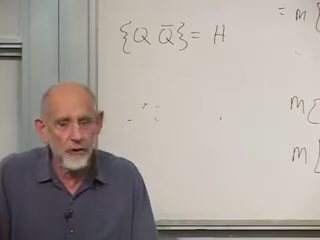
\includegraphics[width=0.62\textwidth]{lecture_05_figure_02.png}
\lectureframe{00:55:46.300}
\caption{Die zentrale Abschlussrelation, wie sie an der Tafel hervorgehoben ist. Die Klammern und \(Q,\bar Q,H\) sind sichtbar; das Komma ergibt sich aus der üblichen Antikommutator-Notation.}
\end{figure}

Der additive Nullpunkt der Energie ist so gewählt, dass der leere Zustand \(H=0\) hat. Beim supersymmetrischen Oszillator ist dies die natürliche Konvention: Die bosonischen und fermionischen Nullpunktsbeiträge heben sich auf. \editorialnote{Die Vorlesung arbeitet direkt mit der gesamten Ruheenergie und stellt keine getrennten Nullpunktsbeiträge dar; die angegebene Konvention macht diese Wahl ausdrücklich.}

Der Hamiltonoperator ist gerade. Er ist außerdem ein Symmetrieerzeuger: Er erzeugt Zeittranslationen. Die ungeraden Erzeuger schließen sich daher untereinander nur dann nicht, wenn man den geraden Erzeuger der Zeittranslation einbezieht.

\begin{classroomqa}
\audiencequestion{Welches Element der Relation ist gerade? Ist es der Hamiltonoperator? \lecturetimestamp{00:58:24}}
\lecturerresponse{Ja. Energie ist eine gewöhnliche Observable, also ist \(H\) gerade. Die Superladung \(Q\) ist ungerade, und das Produkt zweier ungerader Größen ist gerade; folglich kann \(\{Q,\bar Q\}\) gleich \(H\) sein. Ein ungerader und ein gerader Erzeuger stehen durch einen Kommutator in Beziehung, nicht durch einen Antikommutator.}
\end{classroomqa}

\subsection{Vervollständigung der Algebra}

Die Relationen für gleiche Parität folgen unmittelbar:
\begin{equation}
\{Q,Q\}=2Q^2=0,
\qquad
\{\bar Q,\bar Q\}=2\bar Q^2=0,
\end{equation}
Denn \(Q^2\) enthält \(c_-^2\) und \(\bar Q^2\) enthält \(c_+^2\).

Es fehlt noch die Relation mit \(H\). Sei
\begin{equation}
H\ket{E}=E\ket{E}.
\end{equation}
Bei gleichen Massen ersetzt \(Q\) das eine Teilchen durch das andere, ohne die Energie zu ändern. Daher ist \(Q\ket{E}\) entweder null oder ein weiterer Eigenzustand mit demselben Eigenwert:
\begin{equation}
H Q\ket{E}=E Q\ket{E}.
\end{equation}
Andererseits gilt
\begin{equation}
QH\ket{E}=Q(E\ket{E})=E Q\ket{E}.
\end{equation}
Durch Subtraktion folgt
\begin{equation}
[H,Q]\ket{E}=0.
\end{equation}
Wenn die Energieeigenzustände eine vollständige Basis bilden, gilt dies als Operatoridentität:
\begin{equation}
[H,Q]=0,
\qquad
[H,\bar Q]=0.
\end{equation}

\begin{classroomqa}
\audiencequestion{Was geschieht, wenn Boson und Fermion nicht dieselbe Masse haben? \lecturetimestamp{01:01:16}}
\lecturerresponse{Dann ändert sich die Energie beim Ersetzen des einen durch das andere. Die vorgeschlagene Superladung kommutiert folglich nicht mit dem Hamiltonoperator, und die einfache Supersymmetrie geht verloren. Für
\[
H=m_BN_B+m_FN_F,
\]lautet das explizite Ergebnis
\[
[H,Q]=(m_B-m_F)Q.
\]
Es verschwindet genau dann, wenn \(m_B=m_F\) gilt. \editorialnote{Der Kommutator für ungleiche Massen ist die direkte Operatorform des Arguments zur Energieänderung und macht die Bedingung gleicher Massen ausdrücklich sichtbar.}}
\end{classroomqa}

\begin{classroomqa}
\audiencequestion{Kann man das Argument mit den Energieeigenzuständen noch einmal langsamer durchgehen? \lecturetimestamp{01:01:37}}
\lecturerresponse{Man beginne mit \(H\ket{E}=E\ket{E}\). Gleiche Massen bedeuten, dass \(Q\ket{E}\) dieselbe bestimmte Energie \(E\) hat, also gilt \(HQ\ket{E}=EQ\ket{E}\). Für die umgekehrte Reihenfolge erhält man \(QH\ket{E}=QE\ket{E}=EQ\ket{E}\), da \(E\) ein gewöhnlicher Skalar ist. Ihre Differenz verschwindet auf jedem Energieeigenzustand. Aufgrund der Vollständigkeit folgt daraus die Operatorgleichung \([H,Q]=0\).}
\end{classroomqa}

Die vollständige Spielzeugmodell-Algebra lautet somit
\begin{align}
\{Q,\bar Q\}&=H,\\
\{Q,Q\}&=\{\bar Q,\bar Q\}=0,\\
[H,Q]&=[H,\bar Q]=0.
\end{align}
Die Superladungen sind erhaltene ungerade Ladungen. Noch überraschender ist, dass ihre Algebra eine Operation, die den Teilchentyp ändert, mit dem Erzeuger einer Raumzeittranslation verknüpft.

\section{Warum der Hamiltonoperator Zeittranslation bedeutet}

In diesem stark vereinfachten Modell gibt es keine räumliche Koordinate, wohl aber die Zeit. Die Schrödinger-Gleichung lautet
\begin{equation}
i\frac{\partial}{\partial t}\ket{\psi(t)}
=H\ket{\psi(t)}.
\end{equation}

\begin{figure}[H]
\centering
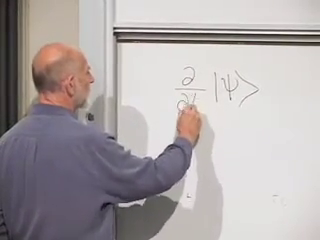
\includegraphics[width=0.56\textwidth]{lecture_05_figure_03.png}
\lectureframe{01:07:26.300}
\caption{Die Zeitableitung neben \(\ket{\psi}\). Die Hand verdeckt einen Teil des Nenners; die vollständige Schrödinger-Gleichung steht oben.}
\end{figure}

Für eine endliche Verschiebung \(\delta\) gilt
\begin{equation}
\ket{\psi(t+\delta)}
=e^{-iH\delta}\ket{\psi(t)}.
\end{equation}
Entwickelt man bis zur ersten Ordnung,
\begin{equation}
\ket{\psi(t+\delta)}
=\left(\mathbf 1-i\delta H\right)\ket{\psi(t)}
+O(\delta^2).
\end{equation}
so ist \(H\) der infinitesimale Erzeuger, der einen Zustand in der Zeit fortentwickelt.

Auch innere Symmetrien wie Isospin und Farbe ändern Teilchenbezeichnungen. Isospin kann Protonen- und Neutronenzustände mischen; Farbrotationen mischen rote, grüne und blaue Quarks. Doch keine Kombination dieser inneren Transformationen verschiebt ein System im Raum oder in der Zeit. Anders ist es bei der Supersymmetrie:
\begin{equation}
\begin{gathered}
\text{odd particle-changing transformation}\\
\mathrel{\stackrel{\{\ ,\ \}}{\Longrightarrow}}\\
\text{time translation}
\end{gathered}
\end{equation}
Das ist der Hinweis darauf, dass die ungeraden Erzeuger selbst Translationen sein könnten, allerdings entlang anderer Koordinaten als der gewöhnlichen.

\section{Superspace}

\subsection{Eine Funktion der Zeit und ungerader Koordinaten}

Führen wir eine Funktion ein:
\begin{equation}
\Psi=\Psi(\theta,\bar\theta,t).
\end{equation}
Im Spielzeugmodell kann sie als Wellenfunktion aufgefasst werden, allgemeiner als Superfeld. Da die ungerade Entwicklung abbricht, gilt
\begin{equation}
\Psi(\theta,\bar\theta,t)
=A(t)+\bar\chi(t)\theta
+\bar\theta\chi(t)+F(t)\bar\theta\theta.
\end{equation}
Dieses einzelne Objekt vereint gerade und ungerade Komponentenfunktionen. \editorialnote{Diese Komponentenentwicklung verwendet das zuvor eingeführte Grassmann-Polynom und gibt den expliziten Standardinhalt einer Funktion auf dem Spielzeug-Superspace wieder.}

Eine gewöhnliche Zeittranslation lässt \(\theta,\bar\theta\) unverändert und bewirkt
\begin{equation}
t\longmapsto t+\delta.
\end{equation}
In erster Ordnung gilt
\begin{equation}
\Psi(\theta,\bar\theta,t+\delta)
=\Psi(\theta,\bar\theta,t)
+\delta\,\partial_t\Psi(\theta,\bar\theta,t).
\end{equation}

\begin{figure}[H]
\centering
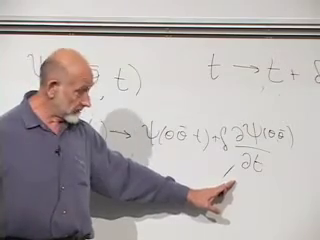
\includegraphics[width=0.72\textwidth]{lecture_05_figure_04.png}
\lectureframe{01:13:15.060}
\caption{An der Tafel steht \(t\to t+\delta\) oberhalb der Änderung erster Ordnung von \(\Psi\); der Ableitungsterm ist direkt angegeben.}
\end{figure}

\subsection{Translation in einer ungeraden Richtung}

Führen wir nun eine Transformation ein, die eine ungerade Koordinate verschiebt:
\begin{equation}
\theta\longmapsto\theta+\epsilon,
\end{equation}
wobei \(\epsilon\) ein weiterer ungerader Grassmann-Parameter ist. Gleichzeitig erhält die Zeit eine gerade nilpotente Verschiebung:
\begin{equation}
t\longmapsto t+i\bar\theta\epsilon.
\end{equation}
Sowohl \(\bar\theta\) als auch \(\epsilon\) sind ungerade; ihr Produkt ist daher gerade und kann konsistent zur geraden Koordinate \(t\) addiert werden.

Verschiebt man den Parameter nach links, gilt
\begin{equation}
i\bar\theta\epsilon=-i\epsilon\bar\theta.
\end{equation}
Die induzierte Variation lautet somit
\begin{align}
\delta_\epsilon\Psi
&=\epsilon\,\partial_\theta\Psi
-i\epsilon\bar\theta\,\partial_t\Psi\\
&=\epsilon q_0\Psi,
\end{align}
wobei
\begin{equation}
q_0=\partial_\theta-i\bar\theta\partial_t.
\end{equation}
Dieser ungerade Differentialoperator erzeugt die kombinierte Verschiebung. Ein kompatibler konjugierter Erzeuger mit linksseitigen Ableitungen ist
\begin{equation}
\bar q_0=-\partial_{\bar\theta}
+i\theta\partial_t.
\end{equation}

Die genauen Vorzeichen hängen davon ab, ob man links- oder rechtsseitige Grassmann-Ableitungen verwendet und wie die Konjugation ungerade Faktoren umordnet. Unabhängig von der Konvention muss der Abschluss auf der Zeittranslation sein. Mit den obigen Definitionen gilt
\begin{align}
\{q_0,\bar q_0\}
&=i\{\partial_\theta,\theta\}\partial_t
+i\{\bar\theta,\partial_{\bar\theta}\}\partial_t\\
&=2i\partial_t.
\end{align}
Der Ableitung-mal-Ableitung-Term verschwindet ebenso wie der quadratische Term in den ungeraden Koordinaten. Die beiden gemischten Terme liefern jeweils \(i\partial_t\).

Da für Zustände im Schrödinger-Bild \(H=i\partial_t\) gilt,
\begin{equation}
\{q_0,\bar q_0\}=2H.
\end{equation}
normieren wir
\begin{equation}
q=\frac{q_0}{\sqrt2},
\qquad
\bar q=\frac{\bar q_0}{\sqrt2},
\end{equation}
so folgt
\begin{equation}
\boxed{\{q,\bar q\}=H.}
\end{equation}
\editorialnote{Die Vorlesung geht die unsicheren Vorzeichen bewusst durch und bemerkt dann einen Faktor zwei. Die angegebene Konvention mit linksseitigen Ableitungen erhält diese Rechnung aus dem Unterricht und legt zugleich eine in sich konsistente Normierung fest. Bei anderen üblichen Konventionen treten Vorzeichen an anderer Stelle auf, nämlich bei den Koordinatenverschiebungen und den Erzeugern.}

\begin{classroomqa}
\audiencequestion{Woher kommt der letzte Faktor zwei im Antikommutator der Superspace-Erzeuger? \lecturetimestamp{01:24:21}}
\lecturerresponse{Es gibt zwei gleich große gemischte Beiträge. Einer stammt von \(\{\partial_\theta,\theta\}=1\), der andere von \(\{\partial_{\bar\theta},\bar\theta\}=1\). Beide multiplizieren die Zeitableitung. Die unnormierten Erzeuger ergeben daher \(2i\partial_t\); ein Faktor \(1/\sqrt2\) in jeder Superladung stellt die frühere Normierung wieder her.}
\end{classroomqa}

\begin{classroomqa}
\audiencequestion{Wurde bei der Konstruktion angenommen, dass \(\epsilon\) klein ist? \lecturetimestamp{01:24:51}}
\lecturerresponse{Entscheidend war die Nilpotenz, nicht ein gewöhnlicher numerischer Betrag. Da \(\epsilon^2=0\) gilt, bricht jede Entwicklung in einer einzelnen Größe \(\epsilon\) nach dem linearen Term ab. Sie infinitesimal oder klein zu nennen, ist eine nützliche Analogie, doch der Abbruch ist exakt.}
\end{classroomqa}

\editorialnote{Grassmann-Parameter besitzen keinen gewöhnlichen positiven Betrag. Ihre Rolle als infinitesimale Parameter ergibt sich aus der Nilpotenz und dem exakten Abbruch der Entwicklung.}

\subsection{Die geometrische Bedeutung}

Die Algebra hat nun zwei gleichwertige Realisierungen. Im Oszillatorbild ersetzen \(Q\) und \(\bar Q\) Fermionen durch Bosonen beziehungsweise Bosonen durch Fermionen. Im geometrischen Bild verschieben \(q\) und \(\bar q\) eine Funktion durch ungerade Richtungen und bewirken zugleich eine gewöhnliche Zeitverschiebung. In beiden Bildern gilt
\begin{equation}
\begin{gathered}
\{\text{supercharge},\text{conjugate supercharge}\}\\
=\text{time-translation generator}.
\end{gathered}
\end{equation}

Der verallgemeinerte Koordinatenraum, der \(t,\theta,\bar\theta\) enthält, heißt Superspace. In einer relativistischen Feldtheorie enthält er auch die gewöhnlichen räumlichen Koordinaten, und die Superladungen schließen sich auf dem vollständigen Raumzeitimpuls \(P_\mu\), nicht nur auf \(H=P_0\). Die Krümmung dieser Struktur führt in Richtung der Supergravitation.

In einer Hinsicht sind Grassmann-Variablen ein effizientes Hilfsmittel, um Bosonen und Fermionen zu verbuchen. In einer anderen sagt die Abschlussrelation etwas wesentlich Tieferes aus: Die Unterscheidung zwischen Teilchentyp und Raumzeitgeometrie ist nicht mehr absolut. Zweimalige Bewegung in ungeraden Richtungen erzeugt Bewegung in einer gewöhnlichen Richtung. Ob die Natur diese Struktur experimentell verwirklicht, ist eine andere Frage als die mathematische Tatsache, dass sie widerspruchsfrei, ökonomisch und bemerkenswert starr ist.
